%Text Books : \cite{royden}
%Module 1: Lebesgue Measure
%Introduction, Lebesgue outer measure, The $\sigma$-algebra of Lebesgue measurable sets, Outer and inner approximation of Lebesgue measurable sets , Countable additivity, continuity and Borel-Cantelli Lemma, Non measureable sets, The Cantor set and Cantor Lebesgue function
%Chapter 2; Sections 2.1 to 2.7 (25 Hours)
%Module 2: Lebesgue Measurable Functions and Lebesgue Integration
%Sums, Products and Compositions, Sequential Pointwise Limits and Simple Approximation, The Riemann Integral, The Lebesgue Integral of a bounded measurable function over a set of finite measure, The Lebesgue Integral of a measurable non-negative function, The General Lebesgue Integral.
%Chapter 3; Sections 3.1 to 3.2, Chapter 4; Sections 4.1 to 4.4(25 Hours) 
%Module 3: General Measure Space and Measureable Functions \& Signed Measures
%Measures and Measurable Sets
%The Hanh and Jordan decompositions, The Caratheodory Measure induced by an outer measure, Measureable functions
%Chapter 17; Sections 17.1 to 17.3, Chapter 18; Section 18.1 upto corollory 7 (20 Hours)
%Module 4: Integration over General Measure Space and Product Measure
%Integration of non-negative meaurable functions, Integration of General Measurable functions, The Radon Nikodym Theorem
%The Theorems of Fubini and Tonelli
%Chapter 18; Sections 18.2 to 18.4, Chapter 20; Section 20.1 (20 Hours)

%Need to work on this
%Module 1 - \cite{royden} 2
%Module 2 - \cite{royden} 3, 4
%Module 3 - \cite{royden} 17, 18
%Module 4 - \cite{royden} 18, 20
%Missing - \cite{royden} 1, 5, 6, 7, 8, 9, 10, 11, 12, 13, 14, 15, 16, 19, 21?

\section{Lebesgue Measure}
\begin{description}
	\item[set function] A function which maps sets into (extended) real numbers.
	\item[$\sigma$-algebra] A family $\mathcal{A}$ of subsets of a nonempty set $X$ such that
	\begin{enumerate}
		\item $\mathcal{A}$ contains the empty set, 
		\item $\mathcal{A}$ contains complement of each of its members and
		\item $\mathcal{A}$ is closed under countable unions.
	\end{enumerate}
	
	From these 3 axioms, we can deduce the following,
	\begin{enumerate}
		\setcounter{enumi}{3}
		\item $\mathcal{A}$ is closed under countable intersections (by de Morgan's laws).
			$$\left( \bigcup_{k = 1}^\infty E_k^c \right)^c = \bigcap_{k=1}^\infty E_k \in \mathcal{A}$$
		\item $E,F \in \mathcal{A} \implies E-F \in \mathcal{A}$ since $E-F = E \cap F^c$
	\end{enumerate}
\end{description}

\begin{definition}[Length of an interval]
	Length is a real valued set function.
	Let $I$ be a bounded interval say $[a,b)$.
	Then its length $l(I)=b-a$ is the difference between endpoints.
	If an interval $I$ is unbounded say $(a,\infty)$, then its length, $l(I) = \infty$.
\end{definition}

\subsubsection{Exercise}
\subsubsection{Techniques in Measure Theory}
	Let $\mathcal{A}$ be a $\sigma$-algebra.
	Let Lebesgue Measure $m : \mathcal{A} \to [0,\infty]$ be countably additive over disjoint collection of sets in $\mathcal{A}$.
\begin{itemize}
	\item Lebesgue Measure $m$ has monotonicity.\\
		$A \subseteq B \implies B = A \cup (B-A)$ is a disjoint union \\
		$\implies m(B) = m(A) + m(B-A) \ge m(A)$
	\item If exists $E \in \mathcal{A}$ such that $m(E) < \infty$, then $m(\phi) = 0$\\
		Suppose $m(\phi) = c$ and $m(E) = k$ where $k < \infty$.
		If $c \ne 0$, then $m(E \cup \phi) = m(E) + m(\phi) = c+k > k = m(E)$ is a contradiction.
	\item $m\left(\displaystyle\bigcup_{k=1}^\infty E_k\right) \le \displaystyle\sum_{k=1}^\infty m(E_k)$\\
		Define $\{ F_k : k \in \mathbb{N} \}$ by $F_k = E_k - \cup_{j = 1}^{k-1} E_j$\\
		Then $F_1 = E_1$, $F_2 = E_2 - E_1$, $F_3 = E_3 - (E_1 \cup E_2)$, \dots\\
		Also $F_k \in \mathcal{A}$ and $F_k \subseteq E_k,\ \forall k \in \mathbb{N}$.
		Thus $m(F_k) \le m(E_k),\ \forall k$
		However, $\cup_{k=1}^\infty E_k = \cup_{k=1}^\infty F_k$\\
		$\implies m\left( \cup_{k=1}^\infty E_k \right) = m \left( \cup_{k=1}^\infty F_k \right) = \displaystyle\sum_{k=1}^\infty m(F_k) \le \displaystyle\sum_{k=1}^\infty m(E_k)$
\end{itemize}

\subsubsection{Counting Measure}
	The counting measure $c : \mathcal{A} \to [0,\infty]$ is a set function which maps sets to their cardinality.
	For example, if $E = \{2,3,4\}$, then $c(E) = 3$.
\begin{itemize}
	\item The counting measure is \textbf{translation invariant} since translation never increases the cardinality of the set.\\
	For example, $5+E = \{7,8,9\}$.
	And $m(5+E) = 3 = m(E)$.
	\item The counting measure is \textbf{countably additive} over disjoint collections since the cardinality of disjoint union of two sets is the sum of their cardinalities.
	\item However, counting measure of (non-degenerate) intervals are $\infty$ which is \textbf{not the same as their length} for bounded intervals.
\end{itemize}

\subsection{Lebesgue Outer Measure}
\begin{description}
	\item[$G_\delta$] A set which is countable intersection of open subsets.
	\item[$F_\sigma$] A set which is countable union of closed subsets.
\end{description}

\subsubsection{Set-theoretic Construction of Lebesgue Measure}
\begin{enumerate}
	\item Construct Lebesgue Outer Measure $m^\ast$ (with Axiom 3 relaxed) \\
		ie, Obtain the underlying relation of the set function
	\item Restrict $m^\ast$ to the $\sigma$-algebra of our interest \\
		ie, Choose a domain so that set function is well defined.
\end{enumerate}
\begin{definition}[Lebesgue Outer Measure]
	Let $A \subset \mathbb{R}$.
	Let $\mathcal{C} = \{ I_k : k \in \mathbb{N}\}$ be an open cover of $A$ such that $I_k$ are non-empty, bounded, open intervals.
	Consider the sum of length of intervals for such covers of $A$.
	(Lebesgue) Outer Measure $m^\ast(A)$ is the infimum of all such sums.
\begin{equation}
	 m^\ast(A) = \inf \left\{ \sum_{k=1}^\infty l(I_k) : A \subset \bigcup_{k=1}^\infty I_k \right\} 
	 \label{eq:outermeasure}
\end{equation}
\end{definition}
\subsection{Properties of Lebesgue Outer Measure}
\begin{enumerate}
	\item Outer Measure of the empty set is zero\\
	Let $\epsilon > 0$.
	Then $\mathcal{C}_\epsilon = \{ (0,\frac{\epsilon}{2^n}) : n \in \mathbb{N} \}$ is an open cover of $\phi$ containing nonempty, bounded, open intervals.
	Clearly, sum of length of intervals in $C_\epsilon = \epsilon$.
	Suppose $m^\ast(\phi) = \delta$ and $\delta > 0$.
	There exists $\epsilon$ such that $0 < \epsilon < \delta$.
	The sum of intervals of $\mathcal{C}_\epsilon$ is less than $\delta$, which is a contradiction by the definition of Outer Measure.
	\item Outer Measure is monotone\\
	Suppose $A \subset B$.
	Then every cover of $B$ is also an  cover of $A$.
	Let $\mathcal{U}$ be the set of all open covers of $A$ with nonempty, bounded intervals and $\mathcal{V}$ be the set of all such open covers of $A$.
	Clearly, $\mathcal{V} \subset \mathcal{U}$.
	We know that, if $A \subset B$, then $\inf{B} \le \inf{A}$.
	Therefore,
	\begin{equation}
		A \subset B \implies m^\ast(A) \le m^\ast(B)
	\end{equation}
	\item Outer Measure of Countable Sets is zero\\
	Let $C$ be a countable set.
	That is, $C = \{ c_k \}_{k=1}^\infty$.\\
	Then $\{ (c_k-\frac{\epsilon}{2^k}, c_k + \frac{\epsilon}{2^k}) \}_{k=1}^\infty$ is cover of $C$ with sum of length of intervals $\epsilon$.
	Thus, for any $\epsilon > 0$, we have $m^\ast(C) \le \epsilon$.
	Thus, $m^\ast(C) = 0$.
	\item Outer Measure of an Interval is its length
	\begin{proof}
		\textbf{Case 1 : Closed, Bounded Interval}
		Let $[a,b]$ be a closed, bounded interval.
		Then for any $\epsilon > 0$, $(a-\epsilon,b+\epsilon)$ is a cover of $[a,b]$.
		Thus, by the definition of outer measure $m^\ast([a,b]) \le b-a+2\epsilon$ since $[a,b] \subset (a-\epsilon,b+\epsilon)$ and $m^\ast$ is monotonic.
		Therefore,
	\begin{equation}
		m^\ast([a,b]) \le b-a
	\end{equation}

	Since $[a,b]$ is closed and bounded, $[a,b]$ is compact.
	And by Heine-Borel theorem, every open cover of $[a,b]$ has a finite subcover.
	Thus, it is sufficient to prove the theorem for finite covers of $[a,b]$.\\

	Let $\mathcal{C}$ be a finite cover of $[a,b]$ with $n$ open intervals.
	Let $(a_1,b_1)$ be an open interval containing $a$ in $\mathcal{C}$.
	Then $a_1 < a < b_1$.
	If $b_1 > b$ then $l(a_1,b_1) > l(a,b)$.
	And $\displaystyle\sum_{i=1}^k l(I_k) \ge l(a_1,b_1) \ge b-a$.

\begin{center}
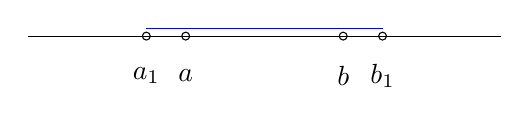
\begin{tikzpicture}
	\draw (-3,0) -- (3,0);
	\draw[blue] (-1.5,0.1) -- (1.5,0.1);
	\draw (-1,0) circle (0.05cm);
	\draw (-1,-0.5) node{$a$};
	\draw (1,0) circle (0.05cm);
	\draw (1,-0.5) node{$b$};

	\draw (-1.5,0) circle (0.05cm);
	\draw (-1.5,-0.5) node{$a_1$};
	\draw (1.5,0) circle (0.05cm);
	\draw (1.5,-0.5) node{$b_1$};
\end{tikzpicture}
\end{center}

	Suppose $b_1 < b$.
	Clearly, $a < b_1$.
	And the cover $\mathcal{C}$ must have an open interval containing $b_1$.
	Otherwise $\mathcal{C}$ is not a cover of $[a,b]$.
	That is, there exists $(a_2,b_2)$ containing $b_1 \in (a,b)$ such that $a_2 < b_1 < b_2$.
	If $b_2 > b$, then $\displaystyle\sum_{i=1}^k l(I_k) \ge l(a_1,b_1) + l(a_2,b_2) \ge l(a_1,b_2) \ge b-a$.

\begin{center}
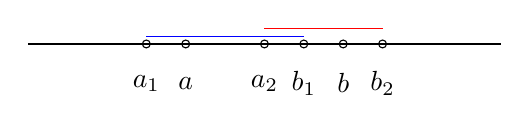
\begin{tikzpicture}
	\draw (-3,0) -- (3,0);
	\draw (-1,0) circle (0.05cm);
	\draw (-1,-0.5) node{$a$};
	\draw (1,0) circle (0.05cm);
	\draw (1,-0.5) node{$b$};

	\draw (-1.5,0) circle (0.05cm);
	\draw (-1.5,-0.5) node{$a_1$};
	\draw (0.5,0) circle (0.05cm);
	\draw (0.5,-0.5) node{$b_1$};
	\draw[blue] (-1.5,0.1) -- (0.5,0.1);

	\draw (0,0) circle (0.05cm);
	\draw (0,-0.5) node{$a_2$};
	\draw (1.5,0) circle (0.05cm);
	\draw (1.5,-0.5) node{$b_2$};
	\draw[red] (0,0.2) -- (1.5,0.2);
\end{tikzpicture}
\end{center}

	Suppose $b_2 < b$.
	Continuing like this we get, $N$ open intervals in $\mathcal{C}$, $\{ (a_k,b_k) : k = 1,2,\cdots,N \} $ such that $a_1 < a < b_1$ and $a_N < b < b_N$ and $a_k < b_{k-1} < b_k$ for all $k$.
	The process should terminate in fintie steps as $\mathcal{C}$ is a finite cover of $[a,b]$.
	Then $\displaystyle\sum_{k=1}^N l(I_k) \ge \displaystyle\sum_{k=1}^N l(a_k,b_k) \ge l(a_1,b_N) \ge b-a$.

\begin{center}
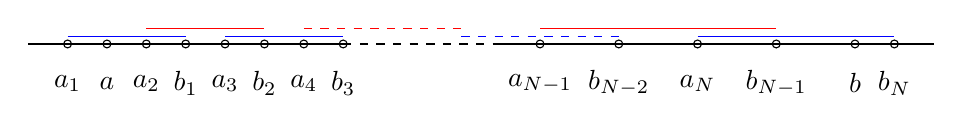
\begin{tikzpicture}
	\draw (-5,0) -- (-1,0);
	\draw[dashed] (-1,0) -- (1,0);
	\draw (1,0) -- (6.5,0);

	\draw (-4,0) circle (0.05cm);
	\draw (-4,-0.5) node{$a$};
	\draw (5.5,0) circle (0.05cm);
	\draw (5.5,-0.5) node{$b$};

	\draw (-4.5,0) circle (0.05cm);
	\draw (-4.5,-0.5) node{$a_1$};
	\draw (-3,0) circle (0.05cm);
	\draw (-3,-0.5) node{$b_1$};
	\draw[blue] (-4.5,0.1) -- (-3,0.1);

	\draw (-3.5,0) circle (0.05cm);
	\draw (-3.5,-0.5) node{$a_2$};
	\draw (-2,0) circle (0.05cm);
	\draw (-2,-0.5) node{$b_2$};
	\draw[red] (-3.5,0.2) -- (-2,0.2);

	\draw (-2.5,0) circle (0.05cm);
	\draw (-2.5,-0.5) node{$a_3$};
	\draw (-1,0) circle (0.05cm);
	\draw (-1,-0.5) node{$b_3$};
	\draw[blue] (-2.5,0.1) -- (-1,0.1);
	
	\draw (-1.5,0) circle (0.05cm);
	\draw (-1.5,-0.5) node{$a_4$};
	\draw[red,dashed] (-1.5,0.2) -- (0.5,0.2);

	\draw (2.5,0) circle (0.05cm);
	\draw (2.5,-0.5) node{$b_{N-2}$};
	\draw[blue,dashed] (0.5,0.1) -- (2.5,0.1);

	\draw (1.5,0) circle (0.05cm);
	\draw (1.5,-0.5) node{$a_{N-1}$};
	\draw (4.5,0) circle (0.05cm);
	\draw (4.5,-0.5) node{$b_{N-1}$};
	\draw[red] (1.5,0.2) -- (4.5,0.2);

	\draw (3.5,0) circle (0.05cm);
	\draw (3.5,-0.5) node{$a_N$};
	\draw (6,0) circle (0.05cm);
	\draw (6,-0.5) node{$b_N$};
	\draw[blue] (3.5,0.1) -- (6,0.1);
\end{tikzpicture}
\end{center}

	Clearly, every open cover of $[a,b]$ contains a finite subcover $\mathcal{C}$, which contains a finite subcover of the form $\{ (a_k,b_k) : k=1,2,\cdots,N \}$ such that $\displaystyle\sum_{k=1}^N l(I_k) \ge b-a$.
	Thus, for any open cover $\displaystyle\sum_{k=1}^\infty l(I_k) \ge b-a$.
	And thus,
	\begin{equation}
		m^\ast([a,b]) \ge b-a
	\end{equation}

	\textbf{Case 2 : Bounded Interval}
	Let $I$ be a bounded interval.
	Then there exists bounded closed intervals $J_1$ and $J_2$ such that $J_1 \subsetneq I \subsetneq J_2$ such that $l(I) - \epsilon < l(J_1)$ and $l(J_2) < l(I)+\epsilon$.
	Suppose $I = (a,b]$, then $J_1 = [a+\frac{\epsilon}{2}, b-\frac{\epsilon}{2}]$ and $J_2 = [a-\frac{\epsilon}{2},b+\frac{\epsilon}{2}]$.\\

	By monotonicity of outer measure, we have $m^\ast(J_1) \le m^\ast(I) \le m^\ast(J_2)$.
	However $m^\ast(J_1) = l(I)-\epsilon$ and $m^\ast(J_2) = l(I)+\epsilon$.
	Thus, $l(I)-\epsilon \le m^\ast(I) \le l(I)+\epsilon$.
	Therefore, $m^\ast(I) = l(I)$.

	\textbf{Case 3 : Unbounded Interval}
	Let $I$ be an unbounded interval.
	Then for any natural number $n$, there exists a closed bounded interval $J$ such that $J \subset I$ and $l(J) = n$.
	And $n = m^\ast(J) \le m^\ast(I),\ \forall n \in \mathbb{N}$.
	Therefore, $m^\ast(I) = \infty = l(I)$. 
	\end{proof}
	\item Outer Measure is translation invariant
	\begin{proof}
	Let $A$ be any set and $y \in \mathbb{R}$.
	Let $\{ I_k : k = 1,2,\dots \}$ be a cover of $A$.
	Then $\{ I_k+y : k = 1,2,\dots \}$ is a cover of $A+y$.
	And $l(I_k) = l(I_k+y)$ for every natural number $k$ and real number $y$.
	Thus, $\displaystyle\sum_{k=1}^\infty l(I_k) = \displaystyle\sum_{k=1}^\infty l(I_k+y)$.
	Clearly, for each cover $\{I_k\}_{k=1}^\infty$ of $A$, there exists a cover $\{ I_k+y \}_{k=1}^\infty$ of $A+y$ containing intevals of same length.
	Therefore, $m^\ast(A) = m^\ast(A+y)$.
	\end{proof}
	\item Outer Measure is countably subadditive
	\begin{proof}
	Let $\{E_k\}_{k=1}^\infty$ be a countable collection of sets.
	It is enough to prove that
		\begin{equation}
			m^\ast \left( \bigcup_{k=1}^\infty E_k \right) \le \sum_{k=1}^\infty m^\ast(E_k)
		\end{equation}
		For each natural number $k$, we have a cover of $E_k$, say $\{ I_{k,i} \}_{i = 1}^\infty$ such that $\displaystyle\sum_{i=1}^\infty I_{k,i} < m^\ast(E_k) + \frac{\epsilon}{2^k}$.
		Suppose that, for some $\epsilon > 0$, $E_k$ doesn't have such a cover, then $m^\ast(E_k) + \frac{\epsilon}{2^k}$ is an upper bound contradicting the assumption that $m^\ast(E_k)$ is the least upper bound.\\

	Clearly,
	\begin{align*}
		m^\ast \left( \bigcup_{i,k = 0}^\infty I_{k,i} \right) \le & \sum_{k=1}^\infty \sum_{i=1}^\infty I_{k,i} \\
		= & \sum_{k=1}^\infty \left( m^\ast(E_k) + \frac{\epsilon}{2^k} \right) \\
		= & \sum_{k=1}^\infty  m^\ast(E_k) + \epsilon
	\end{align*}
	\end{proof}
	\textbf{Note : } Finite subadditivity is a weaker notion than countable subadditivity.
	Since every finite collection is a countable collection.
\end{enumerate}

\subsubsection{Exercise}
\begin{enumerate}
	\setcounter{enumi}{4}
\item Closed Interval $[0,1]$ is uncountable.\\
	Suppose $[0,1]$ is countable, then outer measure of any countable set is zero, $m^\ast([0,1]) = 0$.
		But, $[0,1]$ is an interval and outer measure of an interval is its length, $m^\ast([0,1]) = l([0,1]) = 1$ which is a contradiction.
\item $m^\ast([0,1] - \mathbb{Q}) = 1$
	$$[0,1] = \left( [0,1] \cap \mathbb{Q} \right)\ \cup\ \left( [0,1]\cap \mathbb{Q}^c \right)$$
	Clearly, $m^\ast([0,1]) = 1$.
		And $[0,1] \cap \mathbb{Q}$ is a countable set since $\mathbb{Q}$ is countable.
		And thus has measure zero.
		Thus by countable subadditivity, we have
	$$1 = m^\ast([0,1]) \le m^\ast([0,1] \cap \mathbb{Q}^c) + 0$$
		Thus, $m^\ast([0,1] \cap \mathbb{Q}^c) \ge 1$.
		And $[0,1] \cap \mathbb{Q}^c\ \subset [0,1]$.
		By monotonicity, $m^\ast([0,1] \cap \mathbb{Q}^c) \le m^\ast([0,1]) = 1$.
		Therefore, $m^\ast([0,1] \cap \mathbb{Q}^c) = 1$.
	\item Construction of a $G_\delta$ set containing $E$ % hint : $G_\delta = \cup_{k=1}^\infty F_k$ where
	\item hint : if sum of interval is less than 1.
		Then it is not a cover of $[0,1]$.
	\item hint : $A \cup B = A \cup (B-A) = A \cup (B \cap A^c)$
	\item hint : $A$ and $B$ are separated by distance $\alpha$, thus are disjont.
\end{enumerate}

\subsection{$\sigma$-algebra of Lebesgue Measurable Sets}
	Lebesgue Outer Measure is defined for any subset of real numbers and measure of an interval is its length.
	However, it isn't countable additive.\\


	There exists disjoint sets $A,B$ such that $m^\ast(A\cup B) < m^\ast(A)+m^\ast(B)$.\\
	
	Since countable additivity is a favourable property over countable subadditivity.
	We restrict the family of subsets of real numbers to those subsets that allow countable additivity.
	
\subsubsection{Lebesgue Measurable Set}
\begin{definition}[Measurable Set]
	Let $E$ be a subset of $\mathbb{R}$.
	Then $E$ is Lebesgue measurable if
\begin{equation}
	m^\ast(A) = m^\ast(A \cap E) + m^\ast(A \cap E^c)
	\label{eq:measurable1}
\end{equation}
	for any subset $A$ of $\mathbb{R}$.
\end{definition}

	In other words, $E$ is Lebesgue measurable if $E$ doesn't affect countable additivity of Lebesgue Outer Measure.\\

	We will consider only those subset of real numbers, which won't affect countable additivity.
	These subsets are \textbf{Lebesgue Measurable}.
	And we could show that the collection of all Lebesgue Measurable sets forms a $\sigma$-algebra.
	Clearly, intervals allow countable additivity, thus the Borel Algebra is contained in this $\sigma$-algebra of measurable sets.
\subsubsection{Simplified Condition for Lebesgue Measurability}

We know that Lebesgue Outer Measure has countable subadditivity.
\begin{equation*}
	m^\ast(A) \le m^\ast(A \cap E) + m^\ast(A \cap E^c)
\end{equation*}
Thus, for condition (\ref{eq:measurable1}), it is sufficient to check the following condition,
\begin{equation}
	m^\ast(A) \ge m^\ast(A \cap E) + m^\ast(A \cap E^c)
	\label{eq:measurable2}
\end{equation}

\subsubsection{Properties of Lebesgue Measure}
\begin{enumerate}
	\item Any set of Lebesgue outer measure zero is Lebesgue measurable.
	\begin{proof}
		Let $E$ be a subset of real numbers with outer measure zero.
		Let $A$ be any subset of real numbers.
		Then $A = (A \cap E) \cup (A \cap E^c)$.
		By countable additivity, $m^\ast(A) \le m^\ast(A \cap E) + m^\ast(A \cap E^c)$.
		Since $A\cap E \subset E$, we have by monotonicity $m^\ast(A \cap E) \le m^\ast(E) = 0$.\\


		Again, $A \cap E^c \subset A$ and by monotonicity, $m^\ast(A) \ge m^\ast(A \cap E^c) = 0+m^\ast(A \cap E^c) = m^\ast(A\cap E) + m^\ast(A \cap E^c)$.
		Thus, $E$ is Lebesgue measurable by the simplified condition for measurability.
	\end{proof}

	\item Countable sets are Lebesgue measurable.
	\begin{proof}
	Countable sets are of outer measure zero.
	And sets of outer measure zero are Lebesgue measurable.
	Thus, they are Lebesgue measurable.
	\end{proof}
	\item Finite union of Lebesgue measurable sets is Lebesgue measurable.
	\begin{proof}
		It is enough to prove that if $E_1$ and $E_2$ are Lebesgue measurable, then their union is also Lebesgue measurable.
		Then, by finite mathematical induction, we can prove that the result if true for any finite collection of Lebesgue measurable sets.\\


	Suppose $E_1, E_2$ are measurable sets.
	Since $E_1$ is measurable,
	\begin{equation}
		m^\ast(A) = m^\ast(A \cap E_1) + m^\ast(A \cap E_1^c)
	\end{equation}
	And consider $A \cap E_1^c$ instead of $A$.
	Since $E_2$ is measurable, we get
	\begin{equation}
		m^\ast(A \cap E_1^c) = m^\ast(A \cap E_1^c\cap  E_2) + m^\ast(A \cap E_1^c \cap E_2^c)
	\end{equation}

	We have $(A \cap E_1^c) \cap E_2^c = A \cap (E_1^c \cap E_2^c) = A \cap (E_1 \cup E_2)^c$.
	And $(A \cap E_1) \cup (A \cap E_1^c \cap E_2) = (A \cap E_1) \cup [A \cap (E_2 \cap E_1^c)] = A \cap (E_1 \cup E_2)$.
\begin{center}
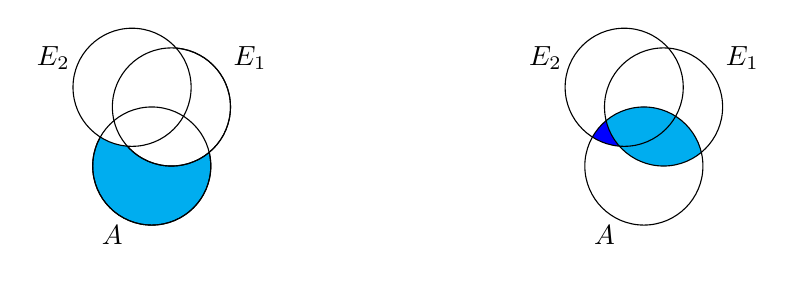
\begin{tikzpicture}[scale=0.25]
	\filldraw[fill = cyan] (0,-1.5) circle (3cm);
	\filldraw[fill = white] (1,1.5) circle (3cm);
	\filldraw[fill = white] (-1,2.5) circle (3cm);
	\draw (0,-1.5) circle (3cm);
	\draw (1,1.5) circle (3cm);
	\draw (-2,-5) node{$A$};
	\draw (5,4) node{$E_1$};
	\draw (-5,4) node{$E_2$};

	\begin{scope}
		\clip (25,-1.5) circle (3cm);
		\fill[blue] (24,2.5) circle (3cm);
	\end{scope}
	\begin{scope}
		\clip (25,-1.5) circle (3cm);
		\fill[cyan] (26,1.5) circle (3cm);
	\end{scope}
	\draw (25,-1.5) circle (3cm);
	\draw (26,1.5) circle (3cm);
	\draw (24,2.5) circle (3cm);
	\draw (23,-5) node{$A$};
	\draw (30,4) node{$E_1$};
	\draw (20,4) node{$E_2$};
\end{tikzpicture}
\end{center}
	\begin{align*}
		m^\ast(A) = & m^\ast(A \cap E_1) + m^\ast(A \cap E_1^c) \\
		= & {\color{blue}m^\ast(A \cap E_1) + m^\ast(A \cap E_1^c \cap E_2)} + m^\ast(A \cap E_1^c \cap E_2^c) \\
		\ge & {\color{blue}m^\ast[A \cap (E_1 \cup E_2)]} + m^\ast[A \cap (E_1 \cup E_2)^c] 
	\end{align*}
	Therefore $E_1 \cup E_2$ is Lebesgue measurable.
		And by finite induction, finite union of measurable sets is also measurable.
	\end{proof}

	\item Lebesgue Measure is finitely additive.\\
		In other words, Suppose $\{E_k\}_{k = 1}^n$ be a finite collection of disjoint, measurable sets.
		Then measure of their union is the sum of measures.
	\begin{proof}
	Let $A$ be any subset of $\mathbb{R}$ and $\{ E_k \}_{k=1}^n$ be a finite collection of disjoint, measurable subsets of $\mathbb{R}$.
	\begin{equation}
		\text{Claim : }	m^\ast \left( A \cap \left[ \bigcup_{k=1}^\infty E_k\right] \right) = \sum_{k=1}^\infty m^\ast (A \cap E_k)
	\end{equation}
	Trivially, the claim is true for $n=1$.
		Suppose the claim is true for $n-1$.
		That is,
	\begin{equation}
		m^\ast \left( A \cap \left[ \bigcup_{k=1}^{n-1} E_k \right] \right) = \sum_{k=1}^{n-1} m^\ast (A \cap E_k)
	\end{equation}
	From set theory we have,
	\begin{align}
		A \cap \left[ \bigcup_{k=1}^n E_k \right] \cap E_n & = A \cap E_n\\
		A \cap \left[ \bigcup_{k=1}^n E_k \right] \cap E_n^c  & = A \cap \left[ \bigcup_{k=1}^{n-1} E_n \right]
	\end{align}
	By measurability of $E_n$, we have
	\begin{align*}
		m^\ast \left( A \cap \left[ \bigcup_{k=1}^n E_k \right] \right) = & m^\ast \left( A \cap \left[ \bigcup_{k=1}^n E_k \right] \cap E_n \right) + m^\ast \left( A \cap \left[ \bigcup_{k=1}^n E_k \right] \cap E_n^c \right)\\
		& = m^\ast \left( A \cap E_n \right) + m^\ast  \left( A \cap \left[ \bigcup_{k=1}^{n-1} E_n \right] \right) \\
		& =  \sum_{k=1}^n m^\ast \left( A \cap E_k \right) \text{, by mathematical induction}
	\end{align*}
	Taking $A = \mathbb{R}$, we get Lebesgue measure is finitely additive.
		That is,
	\begin{equation}
		m^\ast \left( \bigcup_{k=1}^n E_k \right) = \sum_{k=1}^n m^\ast \left( E_k \right)
	\end{equation}
	\end{proof}
	\item Countable union of measurable sets is measurable
	\begin{proof}
		Let $A$ be any subset of $\mathbb{R}$.
		And $\{ E_k \}_{k=1}^\infty$ be a countable collection of disjoint, measurable subsets of $\mathbb{R}$.
		Define $F_n = \cup_{k=1}^n E_k$ and $E = \cup_{k=1}^\infty E_k$.
		Clearly, $F \subset E$ and $F^c \supset E^c$.
		Thus, $m^\ast(A \cap F_n^c) \ge m^\ast(A \cap E^c)$.
	\begin{align*}
		m^\ast(A) & =  m^\ast (A \cap F_n) + m^\ast (A \cap F_n^c) \\
		& \ge m^\ast \left( A \cap \left[ \bigcup_{k=1}^n E_k \right] \right) + m^\ast(A \cap E^c) \\
		& \ge \sum_{k=1}^n m^\ast(A \cap E_k) + m^\ast(A \cap E^c) 
	\end{align*}
	\begin{align*}
		\lim_{n \to \infty} m^\ast(A) & \ge \lim_{n \to \infty} \sum_{k=1}^n m^\ast(A \cap E_k) + m^\ast(A \cap E^c) \\
		m^\ast(A) & \ge \sum_{k=1}^\infty m^\ast(A \cap E_k) + m^\ast (A \cap E^c) \\
		& \ge m^\ast \left( A \cap \left[ \bigcup_{k=1}^\infty E_k \right] \right) + m^\ast(A \cap E^c) \\
		\implies m^\ast(A) & \ge m^\ast (A \cap E) + m^\ast(A \cap E^c)
	\end{align*}
		By above inequality, $E = \cup_{k=1}^\infty E_k$ is measurable.\\

		And, any countable collection of measurable sets can be expressed as a countable collection of disjoint, measurable sets.
		Let $\{ E_k \}_{k=1}^\infty$ be a collection of measurable sets.
		Then, the countable collection, $\{ E_k' \}_{k=1}^\infty$ defined by $E_k'= E_k - \cup_{j=1}^{k-1}E_k$ contains disjoint, measurable\dag\footnote{Suppose $E_1,E_2$ are measurable, then $E_2^c = \mathbb{R} - E_2$ is measurable by the duality of measurability condition.
		And $E_1 \cap E_2^c = E_1-E_2$ is measurable since countable intersection of measurable sets is measurable (by Property 4 and de Morgan's Law).}
	subsets of $\mathbb{R}$.
		Therefore, countable union of measurable sets is measurable.
	\end{proof}
	\item Every interval is Lebesgue measurable.
	\begin{proof}
	It is sufficient to prove that $(a,\infty)$ is measurable.
	Suppose $(a,\infty)$ is measurable for every $a \in \mathbb{R}$.
	Then interval $(a,b)$ is measurable, since $(a,b) = [(a,\infty) \cap (\mathbb{R}-(b,\infty))]-\{b\}$.\\


	Let $A$ be any subset of $\mathbb{R}$.
	Define $A_1 = A\cap (-\infty,a)$ and $A_2 = A \cap (a,\infty)$ such that $A-\{a\} = A_1 \cup A_2$ and $A_1 \cap A_2 = \phi$.
	And the interval $(a,\infty)$ is measurable only if 
	\begin{equation}
		m^\ast(A) \ge m^\ast(A \cap (a,\infty)) + m^\ast(A \cap (a,\infty)^c) = m^\ast(A_1)+m^\ast(A_2)
		\dag\footnote{We have, $m^\ast(A \cap (-\infty,a]) = m^\ast(A \cap (-\infty,a)$ since removing finite number of points from a subset of $\mathbb{R}$ won't affect its measure.}
	\end{equation}
	Let collection $\{ I_k \}_{k=1}^\infty$ be a countable cover of $A$.
		Then collection $\{ I_k' \}_{k=1}^\infty$ defined by $I_k' = I_k \cap (a,\infty)$ is a cover of $A_1$.
		And collection $\{I_k''\}_{k=1}^\infty$ defined by $I_k'' = I_k \cap (-\infty,a)$ is a cover of $A_2$.\\

	Clearly, $m^\ast(A_1) \le \displaystyle\sum_{k=1}^\infty l(I_k')$ and $m^\ast(A_2) \le \displaystyle\sum_{k=1}^\infty l(I_k'')$.
	\begin{align*}
		m^\ast(A_1)+m^\ast(A_2) & \le \sum_{k=1}^\infty l(I_k') + \sum_{k=1}^\infty l(I_k'') \\
		& \le \sum_{k=1}^\infty l(I_k') + l(I_k'') \\
		& \le \sum_{k=1}^\infty l(I_k) \le m^\ast(A)
	\end{align*}
		Thus, $(a,\infty)$ is measurable.
		Therefore, every interval is measurable.
	\end{proof}
	\item $\sigma$-algebra of Lebesgue measurable sets $\mathcal{M}$ contains Borel Sets $\mathcal{B}$.
	\begin{equation}
		\mathcal{B} \subset \mathcal{M}
	\end{equation}
	\begin{proof}
	The Borel algebra $\mathcal{B}$ is the $\sigma$-algebra containing all intervals.
		We have proved that, every intervals are measurable.
		Also, we have proved that the set of all measurable subsets of $\mathbb{R}$ is a $\sigma$-algebra as complements of measurable sets are measurable by duality of the condition and countable union of measurable sets are also measurable.
		Therefore, every borel set is measurable.
		Clearly, $G_\delta$ and $F_\sigma$ are borel sets and are measurable.
	\end{proof}
	\item Lebesgue Measurability is translation invariant.
	\begin{proof}
		Let $E$ be a measurable set.
		Let $A$ be any subset of $\mathbb{R}$ and $y \in \mathbb{R}$.
		Then,
	\begin{align*}
		m^\ast(A) & = m^\ast(A-y)\\
		& = m^\ast((A-y) \cap E) + m^\ast((A-y) \cap E^c)\\
		& = m^\ast(A \cap (E+y)) + m^\ast(A \cap (E+y)^c)
	\end{align*}
		Thus, $E+y$ is measurable.
		And measurability is traslation invariant.
	\end{proof}
\end{enumerate}

\subsubsection{Exercise}
\begin{enumerate}
	\setcounter{enumi}{10}
	\item Let $\mathcal{A}$ be the $\sigma$-algebra containing all intervals of the form $(a, \infty)$.
		Every interval has one of the four forms,
	\begin{align}
		(a,b] = & (a,\infty) \cap (b,\infty)^c \\
		(a,b) = & (a,\infty) \cap \left[\bigcap_{k=1}^\infty \left(b-\frac{1}{k},\infty\right)\right]^c \\
		[a,b] = & \left[ \bigcap_{k=1}^\infty \left(a-\frac{1}{k},\infty\right)\right] \cap (b,\infty)^c \\
		[a,b) = & \left[\bigcap_{k=1}^\infty \left(a-\frac{1}{k},\infty\right)\right] \cap \left[ \bigcap_{k=1}^\infty \left(b-\frac{1}{k},\infty\right)\right]^c
	\end{align}
\item \textbf{Borel sets} is the $\sigma$-algebra containing all open intervals.
	The equations from previous equations are sufficient.
	However, we have a simpler form for closed intervals, $[a,b]$.
	\begin{align}
		[a,b] = & \left[(-\infty,a) \cup (b,\infty) \right]^c 
	\end{align}
		Clearly, every interval is a borel set.
	\item
	\begin{itemize}
		\item $C \in F_\sigma \implies C = \bigcup_{k=1}^\infty C_k \implies \bigcup_{k=1}^\infty \left(C_k+y\right) = C+y \in F_\sigma$
		\item $O \in G_\delta \implies O = \bigcap_{k=1}^\infty O_k \implies \bigcup_{k=1}^\infty \left( O_k+y \right) =  O+y \in G_\delta$
		\item $m^\ast(E) = 0 \implies 0 = \inf\{\sum_{k=1}^\infty l(I_k)\} = \inf\{\sum_{k=1}^\infty l(I_k+y)\} \implies  m^\ast(E+y) = 0$
	\end{itemize}
	\item A subset $E$ has positive measure if and only if it has a bounded subset of positive measure.
		$$m^\ast(E) > 0 \iff \exists \text{ bounded subset }F \subset E,\text{ such that } m^\ast(F) > 0$$
		\textbf{Sufficient Part :} By monotonicity, $F \subset E \implies m^\ast(F) \le m^\ast(E)$.
		And $m^\ast(F) > 0 \implies 0 < m^\ast(F) \le m^\ast(E)$.\\
		\textbf{Necessary Part :}
	\item 
\end{enumerate}

\subsection{Outer and Inner Approximation}
\begin{definition}[Excision Property]
Let $A$ be a measurable set of finite measure and $A \subset B$.
	Then,
\begin{equation}
	m^\ast(B \sim A) = m^\ast(B) - m^\ast(A)
\end{equation}
\begin{proof}
\begin{align*}
	m^\ast(B) = & m^\ast(B \cap A) + m^\ast(B \cap A^c) \\
	= & m^\ast(A) + m^\ast(B \sim A) \\
	\implies m^\ast(B \sim A) = & m^\ast(B) - m^\ast(A)
\end{align*}
\end{proof}
\end{definition}

\begin{theorem}[approximation]
	The following conditions are equivalent to measurability of $E$
\begin{enumerate}
	\item $\forall \epsilon > 0$, there is an open set $\mathcal{O}$ containing $E$ for which $m^\ast(\mathcal{O}\sim E) < \epsilon$.
	\item There is a $G_\delta$ set $G$ containining $E$ such that $m^\ast(G \sim E) = 0$.
	\item $\forall \epsilon > 0$, there is a closed set $F$ contained in $E$ such that $m^\ast(E\sim F) = 0$.
	\item There is an $F_\sigma$ set $F$ contained in $E$ sucht hat $m^\ast(E \sim F) = 0$.
\end{enumerate}
\end{theorem}

\textbf{Note :} Equivalent conditions 1 \& 2 are about outer approximation of a measurable set and 3 \& 4 are about inner approximation of a measurable set.\\

\begin{proof}
\subsubsection*{Measurability $\implies$ Open set - Outer approximation}
	Suppose that $E$ is measurable.
	And let $\epsilon > 0$.\\


	\textbf{Case 1 :} Suppose $m^\ast(E) < \infty$.
	By definition of outer measure, there exists an open cover $\{ I_k \}_{k=1}^\infty$ such that $\displaystyle\sum_{k=1}^\infty l(I_k) <  m^\ast(E)+\epsilon$.\\

	Define $\mathcal{O} = \displaystyle\bigcup_{k=1}^\infty I_k$.
	Then $\mathcal{O}$ is an open set containing $E$ and thus measurable.
	Also, $m^\ast(\mathcal{O}) \le \displaystyle\sum_{k=1}^\infty l(I_k) < m^\ast(E) + \epsilon$.
	Therefore, by excision property we have $m^\ast(\mathcal{O} \sim E) = m^\ast(\mathcal{O}) - m^\ast(E) < \epsilon$. \\

	\textbf{Case 2 :} Suppose $m^\ast(E) = \infty$.
	Without loss of generality, $E$ may be written as countable union measurable sets $\{ E_k \}_{k=1}^\infty$ of finite measure.\\

	By case 1, for every $k$, there exists $\mathcal{O}_k$ for each $E_k$ of finite measure such that $m^\ast(\mathcal{O}_k \sim E_k) < \frac{\epsilon}{2^k}$.
	Define $\mathcal{O} = \displaystyle\bigcup_{k=1}^\infty \mathcal{O}_k$.
	Then $\mathcal{O}$ is open, contains $E$ and 
	\begin{align*}
		m^\ast(\mathcal{O} \sim E) = & m^\ast\left(\bigcup_{k=1}^\infty \mathcal{O}_k \sim E \right) \\
		\le & m^\ast \left(\bigcup_{k=1}^\infty \mathcal{O}_k \sim E_k \right) \\
		\le & \sum_{k=1}^\infty m^\ast(\mathcal{O}_k \sim E_k) = \epsilon \sum_{k=1}^\infty \frac{1}{2^k} = \epsilon
	\end{align*}

\subsubsection*{Open, Outer approximation $\implies G_\delta$, Outer approximation }
	Let $E$ be a subset of real numbers such that measure of $E$ has an open set inner approximation.
	That is, for every $\epsilon > 0$, there exits an open set $\mathcal{O}$ such that $m^\ast(\mathcal{O} \sim E) < \epsilon$.\\

	Let $\mathcal{O}_k$ be open sets such that $m^\ast(\mathcal{O}_k \sim E) < \frac{1}{k}$.
	Define $G = \displaystyle\bigcap_{k=1}^\infty \mathcal{O}_k$.
	Then, $G$ is a $G_\delta$ set containing $E$.
	And $G \sim E \subset \mathcal{O}_k \sim E$.
	Thus, by monotonicity, $m^\ast(G \sim E) \le m^\ast(\mathcal{O}_k \sim E) < \frac{1}{k}$.
	Thus, we have a $G_\delta$ set $G$ containing $E$ such that $m^\ast(G \sim E) = 0$.

\subsubsection*{$G_\delta$-Outer approximation $\implies$ Measurability}
	We have, $m^\ast(G \sim  E) = 0$.
	Since every set of measure zero is measurable, $G \sim E$ is measurable.
	And its complement $(G \sim E)^c$ is also measurable.
	Also we have, $G$ is a $G_\delta$ set, thus a borel set and hence measurable.\\

	Clearly,we have $E = G \cap (G \sim E)^c$.
	And therefore, $E$ is measurable.

\subsubsection*{Open, Outer approximation $\iff$ Closed, Inner approximation}
	By duality of measurability, $E$ is measurable if and only if $E^c$ is measurable.
	And by de Morgan's Law, we have $E^c$ has an open set - outer approximation $\mathcal{O}$ if and only if $E$ has a closed set - inner approximation $\mathcal{O}^c$.
	$$ m^\ast(\mathcal{O} \sim E^c) < \epsilon \iff m^\ast(E \sim \mathcal{O}^c) < \epsilon $$

\subsubsection*{$G_\delta$-Outer approximation $\iff F_\sigma$-Inner approximation}
	Again, by duality of measurability and de Morgan's Law, we have $E^c$ has a $G_\delta$-outer approximation $G$ if and only if $E$ has an $F_\sigma$-inner approximation $F$.
	$$ m^\ast(G \sim E^c) < \epsilon \iff m^\ast(E \sim F) < \epsilon $$
\end{proof}

\begin{theorem}
	Let $E$ be a measurable set of finite measure.
	Then for any $\epsilon > 0$, there exists a finite collection of disjoint open sets $\{ I_k \}_{k=1}^n$ such that  $\mathcal{O} = \displaystyle\bigcup_{k=1}^n I_k$ and $m^\ast(\mathcal{O} \sim E) + m^\ast(E-\mathcal{O}) < \epsilon$.
\end{theorem}
\begin{proof}
	Since $E$ is measurable, by outer approximation theorem we have an open set $U$ such that $E \subset U$ and 
	\begin{equation*}
		m^\ast(U \sim E) < \frac{\epsilon}{2}
	\end{equation*}

	\begin{align*}
		U =  & (U \cap E) \cup (U \cap E^c)
		\intertext{Since $E$ is measurable, $m^\ast(E) < k$}
		m^\ast(U) = &  m^\ast(U \cap E) + m^\ast(U \cap E^c) \\
		= & m^\ast(E) + m^\ast(U \sim E)
		\intertext{Since $E$ has finite measure}
		m^\ast(U) = & m^\ast(E) + m^\ast(U \sim E) \\
		< & k+\frac{\epsilon}{2} < \infty
	\end{align*}
	That is, $U$ is of finite measure. \\

	Since $U$ is open, $U$ is countable\dag\footnote{
		By definition, \textbf{Open sets} are countable union of disjoint, open intervals}
	union of a disjoint collection of open intervals, say $\{ I_k \}_{k=1}^\infty$. Clearly,
	\begin{align*}
		\sum_{k=1}^n l(I_k) & \le \sum_{k=1}^\infty \le m^\ast(U) < \infty \\
		\sum_{k=1}^\infty l(I_k) & < \infty 
		\intertext{ By characterisation of series convergence, there exists an integer $n$ such that,}
		\sum_{k=n+1}^\infty l(I_k) & < \frac{\epsilon}{2}
	\end{align*}
	Define $\mathcal{O} = \displaystyle\bigcup_{k=1}^n I_k$.
	Since $\mathcal{O} \sim E \subset U \sim E$, by monotonicity we have 
	\begin{equation}
		m^\ast(\mathcal{O} \sim E) \le m^\ast(U \sim E) < \frac{\epsilon}{2}
	\end{equation}

	Since $E \subset U$, we have $E \sim \mathcal{O} \subset U \sim \mathcal{O} = \displaystyle\bigcup_{k=1}^n I_k$.
	And clearly, 
	\begin{equation*}
		U \sim \mathcal{O} = \displaystyle\bigcup_{k=1}^\infty I_k \sim \displaystyle\bigcup_{k=1}^n I_k = \displaystyle\bigcup_{k=n+1}^\infty I_k
	\end{equation*}
	\begin{align}
		\text{Thus, } m^\ast(E \sim \mathcal{O}) \le & m^\ast(U \sim \mathcal{O}) \le \sum_{k=n+1}^\infty l(I_k) < \frac{\epsilon}{2} 
		\intertext{Therefore,}
		m^\ast(E \sim \mathcal{O}) + m^\ast(\mathcal{O} \sim E) < & \epsilon \nonumber
	\end{align}
\end{proof}

\subsubsection{Exercise}

\begin{enumerate}
	\setcounter{enumi}{16}
\item Let $\epsilon > 0$ and $E$ is measurable.
	Then there exists open set $\mathcal{O}$ and closed set $F$ such that $F \subset E \subset \mathcal{O}$, $m^\ast(E \sim F) < \frac{\epsilon}{2}$ and $m^\ast(\mathcal{O} \sim E) < \frac{\epsilon}{2}$.
	Clearly, $\mathcal{O} \sim E$ and $E \sim F$ are disjoint and $\mathcal{O} \sim F = (\mathcal{O} \sim E) \cup (E \sim F)$.
		Thus by monotonicity of Lebesgue outer measure, we have $m^\ast(\mathcal{O} \sim F) \le m^\ast(\mathcal{O} \sim E) + m^\ast(E \sim F) < \epsilon$.
\item
 Suppose $E$ has finite outer measure.
	\dag\footnote{
		$E$ has finite outer measure does not imply $E$ is bounded or measurable.}\\
	\textbf{$G_\delta$ set : }
	Let $\epsilon > 0$.
	Then by the definition of outer measure, there exists a cover $\{ I_k \}_{k=1}^\infty$ of $E$ such that $\displaystyle\sum_{k=1}^\infty l(I_k) < m^\ast(E) - \frac{\epsilon}{2}$.
	Define $G = \displaystyle\bigcup_{k=1}^\infty I_k$.
	Then $G$ is a $G_\delta$ set and $m^\ast(G) \le \displaystyle\sum_{k=1}^\infty l(I_k) < m^\ast(E) - \frac{\epsilon}{2}$.\\

	\textbf{$F_\sigma$ set : }
		%---yet to update---
\item
 	Let $E$ be a set of finite outer measure.
	Suppose $E$ is not measurable.
	And $\mathcal{O}$ be an open set containing $E$.
	Then $\mathcal{O} = (\mathcal{O} \sim E) \cup E$.
		By monotonicity, $m^\ast(\mathcal{O}) \textcolor{red}{ \le } m^\ast(\mathcal{O} \sim E) + m^\ast(E)$
		\dag\footnote{\textcolor{red}{I am not able to change $\le$ into $<$} as non-measurability doesn't mean that for this particular $\mathcal{O}$ the sum of outer measures should be greater. There may be a better proof.}.
	Since $m^\ast(E)$ is finite, we have $m^\ast(\mathcal{O}) - m^\ast(E) \le m^\ast(\mathcal{O} \sim E)$.
\item  Let $E$ be a set of finite outer measure.
	Suppose $E$ is measurable.
	Let $(a,b)$ be any open, bounded interval.
	Then by the definiton of measurability, $b-a = m^\ast(a,b) = m^\ast((a,b) \cap E) + m^\ast((a,b) \cap E^c)$.
%	Suppose $m^\ast(\mathcal{O}) = m^\ast(\mathcal{O} \cap E) + m^\ast(\mathcal{O} \cap E^c)$ for every open, bounded interval $\mathcal{O}$.
\item  
 	A subet $E$ is measurable if there exists a $G_\delta$ set $G$ containing $E$ such that $m^\ast(G \sim E) = 0$.
	Suppose $E_1$ and $E_2$ are measurable sets.	
	Then, we have $G_\delta$ sets $G_1$ and $G_2$.
	And two countable family of open intervals $\{\mathcal{O}_{1,k}\}_{k=1}^\infty$ and $\{ \mathcal{O}_{2,k}\}_{k=1}^\infty$ such that $\cap \mathcal{O}_{1,k} = G_1$ and $\cap \mathcal{O}_{2,k} = G_2$.
	Let $\mathcal{O} = \{ \mathcal{O}_k \}_{k=1}^\infty$ be collection of open intervals in $\mathcal{O}_1$ and $\mathcal{O}_2$.
	Define $G = \cap_{k=1}^\infty \mathcal{O}_k$.
	Then, $E = E_1 \cup E_2 \subset G_1 \cup G_2 = G$.
	Since $G \sim E = (G_1 \sim E_1) \cup (G_2 \cup E_2)$, by monotonicity of outer measure we have $m^\ast(G \sim E) \le m^\ast(G_1 \sim E_1) + m^\ast(G_2 \sim E_2) = 0$.
\item
	Let $m^{\ast\ast}$ be a non-negative set function defined by $m^{\ast\ast}(A) = \inf \{ m^\ast(\mathcal{O}) : A \subset \mathcal{O}, \mathcal{O} \text{ is open} \}$.
	Suppose $E$ is measurable.
	Then, by open set - outer approximation theorem
	we have $m^\ast(E) \le m^{\ast\ast}(E) < m^\ast(E) + \epsilon$ for any $\epsilon > 0$.
	Thus, $m^{\ast\ast}(E) = m^\ast(E)$. \\

	In other words, for measurable sets $m^\ast$ and $m^{\ast\ast}$ are the same.
\item  
	Let $m^{\ast\ast\ast}$ be a non-negative set function defined by $m^{\ast\ast\ast}(E) = \sup \{ m^\ast(F) : F \subset E, F \text{ is closed } \}$.
	Let $E$ be measurable set.
	Then, by closed set - inner approximation theorem
	we have $m^\ast(E) \ge m^{\ast\ast\ast}(E) > m^\ast(E)-\epsilon$.\\

	In other words, for measurable sets $m^\ast$ and $m^{\ast\ast\ast}$ are the same.
\end{enumerate}
\subsection{Further Properties}
\subsubsection{Countable Subadditivity}
\begin{theorem}
	The set function Lebesgue measure defined on $\sigma$ algebra of measurable sets
	\begin{enumerate*}
		\item assigns length to any interval, 
		\item is translation invariant, and
		\item is countably additive.
	\end{enumerate*}
\end{theorem}
\begin{proof}
\textbf{Length of interval}\\
	Let $E$ be an interval, then $E$ belongs to the $\sigma$ algebra of measurable sets as Borel sets are measurable.
	Also, we have $m^\ast(E) = m(E)$ for any measurable set $E$.
	And outer measure $m^\ast$ of an interval is its length.
	Therefore, Lebesgue measure of any interval is its length.\\

	\textbf{Translation invariant}\\
	Let $E$ be a measurable set.
	We have, $E+y$ is also measurable.
	Since $E+y$ is measurable and outer measure is translation invariant, we have $m^\ast(E) = m^\ast(E+y) = m(E+y)$.
	Clearly, $m(E) = m(E+y)$.\\

	\textbf{Countably additive}
	\footnote{ A real-valued set function $m$ is countably additive if $m(\cup_{k=1}^\infty E_k) = \sum_{k=1}^\infty m(E_k)$ for any disjoint family of sets $\{E_k\}$.}\\
	Let $\{ E_k \}_{k=1}^\infty$ be a countable family of disjoint, measurable sets.
	Lebesgue outer measure is countably subadditive and countable union of measurable sets is also measurable.
	Thus we have,
	\begin{equation*}
	 	m \left( \bigcup_{k=1}^\infty E_k \right) \le \sum_{k=1}^\infty m(E_k)
	\end{equation*}
	Since Lebesgue measure is finitely additive we have,
	\begin{align*}
		m \left( \bigcup_{k=1}^\infty E_k \right) \ge m \left( \bigcup_{k=1}^n E_k \right) = & \sum_{k=1}^n m(E_k)\\
		\lim_{n \to \infty} m \left( \bigcup_{k=1}^\infty E_k \right) \ge \lim_{n \to \infty} m \left( \bigcup_{k=1}^n E_k \right) = & \lim_{n \to \infty} \sum_{k=1}^n m(E_k)\\
	 	\implies m \left( \bigcup_{k=1}^\infty E_k \right) \ge & \sum_{k=1}^\infty m(E_k)
	\end{align*}
	Therefore, Lebesgue measure is countably additive.
	\begin{equation*}
	 	m \left( \bigcup_{k=1}^\infty E_k \right) = \sum_{k=1}^\infty m(E_k)
	\end{equation*}
\end{proof}
\subsubsection{Continuity}
\begin{theorem}[continuity]
	Let $m$ be Lebesgue measure.
\begin{enumerate}
	\item
	Suppose $\{ A_k \}_{k=1}^\infty$ be an ascending
	\footnote{$\{A_k\}$ is ascending if $A_1 \subset A_2 \subset \dots$}
	collection of measurable sets.
	Then, 
	\begin{equation}
		m \left( \bigcup_{k=1}^\infty A_k \right) = \lim_{k \to \infty} m(A_k)
	\end{equation}
	\item
	Suppose $\{ B_k \}_{k=1}^\infty$ be an descending
	\footnote{$\{A_k\}$ is ascending if $B_1 \supset B_2 \supset \dots$}
	collection of measurable sets and $m(B_1) < \infty$.
	Then, 
	\begin{equation}
		m \left( \bigcap_{k=1}^\infty B_k \right) = \lim_{k \to \infty} m(B_k)
	\end{equation}
	\end{enumerate}
\end{theorem}
\begin{proof}
\end{proof}
\subsubsection{Borel-Cantelli Lemma}
\begin{lemma}[Borel-Cantelli]
	Let $\{E_k\}_{k=1}^\infty$ be a countable colection of measurable sets for which $\sum_{k=1}^\infty m(E_k) < \infty$.
	Then, almost all $x \in \mathbb{R}$ belongs to at most finitely many of the $E_k$s.
\end{lemma}
\begin{proof}
\end{proof}
